\documentclass{article}
\usepackage{graphicx}
\graphicspath{{./Pictures/}}
\usepackage[table,xcdraw]{xcolor}

\title{My first chapter}
\author{Wojciech Łabędź}
\date{3.11.2022}


\begin{document}
\maketitle
\section{Photo}
\begin{center}
\begin{figure}[h!]
  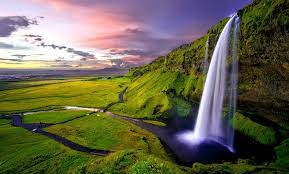
\includegraphics[scale=1.2]{Pictures/iceland.jpg}
  \caption{Iceland}
  \label{iceland_figure}
\end{figure}
\end{center}
\section{Mathematical expression}

\[\sum_{n=1}^{\infty} 2^{-n} =1\]
\pagebreak

\section{Lists}

This is an unordered list:
\begin{itemize}
    \item Item 1
    \item Item 2
    \item Item 3
    \item Item 4
\end{itemize}

This is an ordered list:
\begin{enumerate}
    \item Item1
    \item Item2
    \item Item3
    \item Item4
\end{enumerate}

\begin{table}[]
\begin{tabular}{c|c|c|c|}
\cline{2-4}
\multicolumn{1}{l|}{}                        & \cellcolor[HTML]{9698ED}Column 1 & \cellcolor[HTML]{9698ED}Column 2 & \cellcolor[HTML]{9698ED}Column 3 \\ \hline
\multicolumn{1}{|c|}{\cellcolor[HTML]{9698ED}Row 1} & 123 & 132 & 444 \\ \hline
\multicolumn{1}{|c|}{\cellcolor[HTML]{9698ED}Row 2} & 233 & 122 & 198 \\ \hline
\end{tabular}
\caption{A sample table}
\label{table_1}
\end{table}

\section{Text}
\underline{\textbf{This}} is a sample text divided into \emph{two paragraphs}. \textbf{This} is a sample text divided into \emph{two paragraphs}. \underline{\textbf{This}} is a sample text divided into \emph{two paragraphs}.\par \textbf{This} is a sample text divided into \emph{two paragraphs}. \underline{\textbf{This}} is a sample text divided into \emph{two paragraphs}. \textbf{This} is a sample text divided into \emph{two paragraphs}.
\end{document}
